\section{Introduction}

The accurate determination of initial conditions is crucial when constructing MAD-X lattice models for transfer lines. Unlike circular machines with inherent periodicity, linear lattices require explicit specification of these conditions. The CERN Proton Synchrotron (PS), featuring two extraction lines (F16 and F61), presents unique challenges due to its combined function magnets and strong stray fields.
\\
\\
One approach to determine the initial conditions at the start of a transfer line, such as F61, is to track the particle within the PS ring and store the beam condition at the junction between the PS and the transfer line for use as initial conditions. However, this method encounters challenges in the PS where the particles travel through the combined function magnets of the PS which exhibit strong stray fields. Stray fields are unwanted magnetic fields that extend beyond the intended region, affecting beam dynamics. Complications are further exacerbated by the necessity of extracting through the magnet's transverse plane resulting in a maximal impact from the stray fields. As a result, the beam conditions at extraction remain hard to characterise.
\\
\\
To address these challenges, we propose two methodologies for determining initial conditions through the stray fields:
\begin{enumerate}
    \item{Simulation of the main unit and associated stray fields (elaborated in Section \ref{section:simulation}).}
    \item{Empirical measurements (detailed in Section \ref{section:Empirical_measurements}).}
\end{enumerate}


\subsection{Stray Fields and Field Maps}
\subsubsection{PS Main Units}

The PS is composed of 100 combined-function Main Units (MU) magnets that produce dipolar and quadrupolar fields simultaneously to provide strong focusing. An example of such a magnet is shown in Fig. \ref{fig:combined_fuction_magnet}. Each magnet is divided into two half-units, having quadrupole gradients of opposite polarity. Half-units are composed of five blocks, either closed (focusing) or open (defocusing), see Fig. \ref{fig:combined_fuction_magnet} and \ref{fig:vector_flow}.
\\

\begin{figure}[H]
\centering
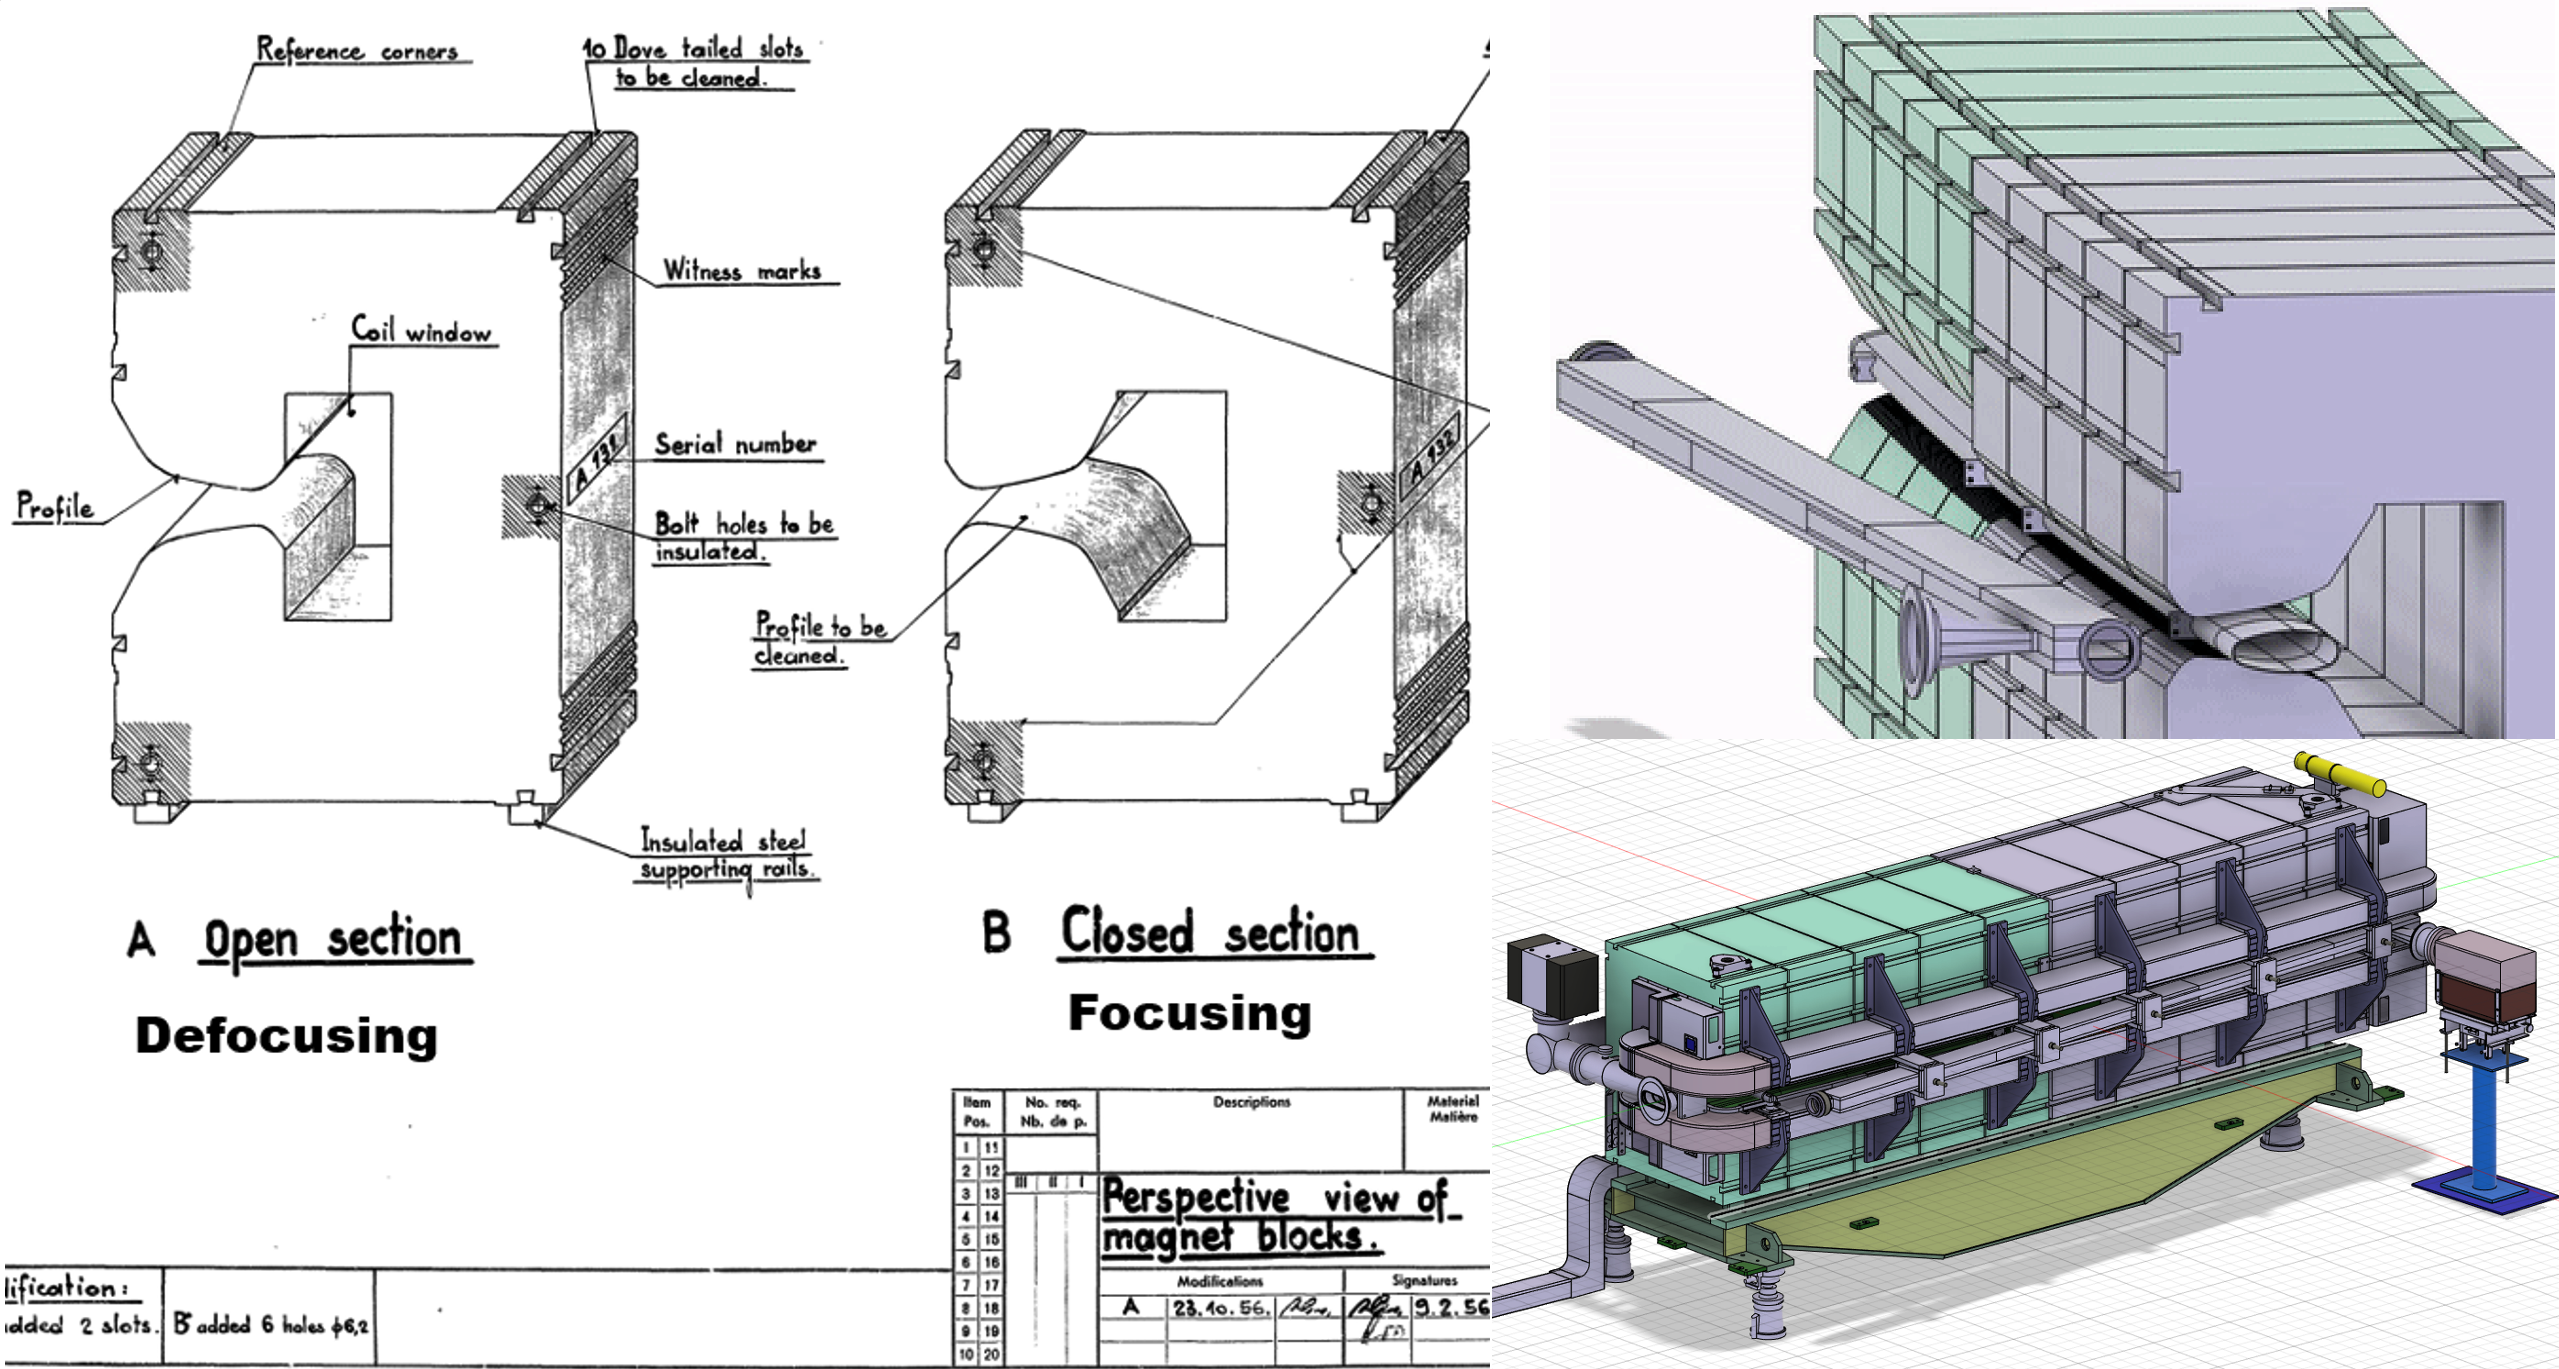
\includegraphics[width=1.0\textwidth]{01_Introduction/images/combined_function_magnets.png}
\caption{MU63 combined-function magnet, highlighting the shim-covered extraction vacuum chamber for the F61 extraction.}
\label{fig:combined_fuction_magnet}
\end{figure}

\begin{figure}[H]
\centering
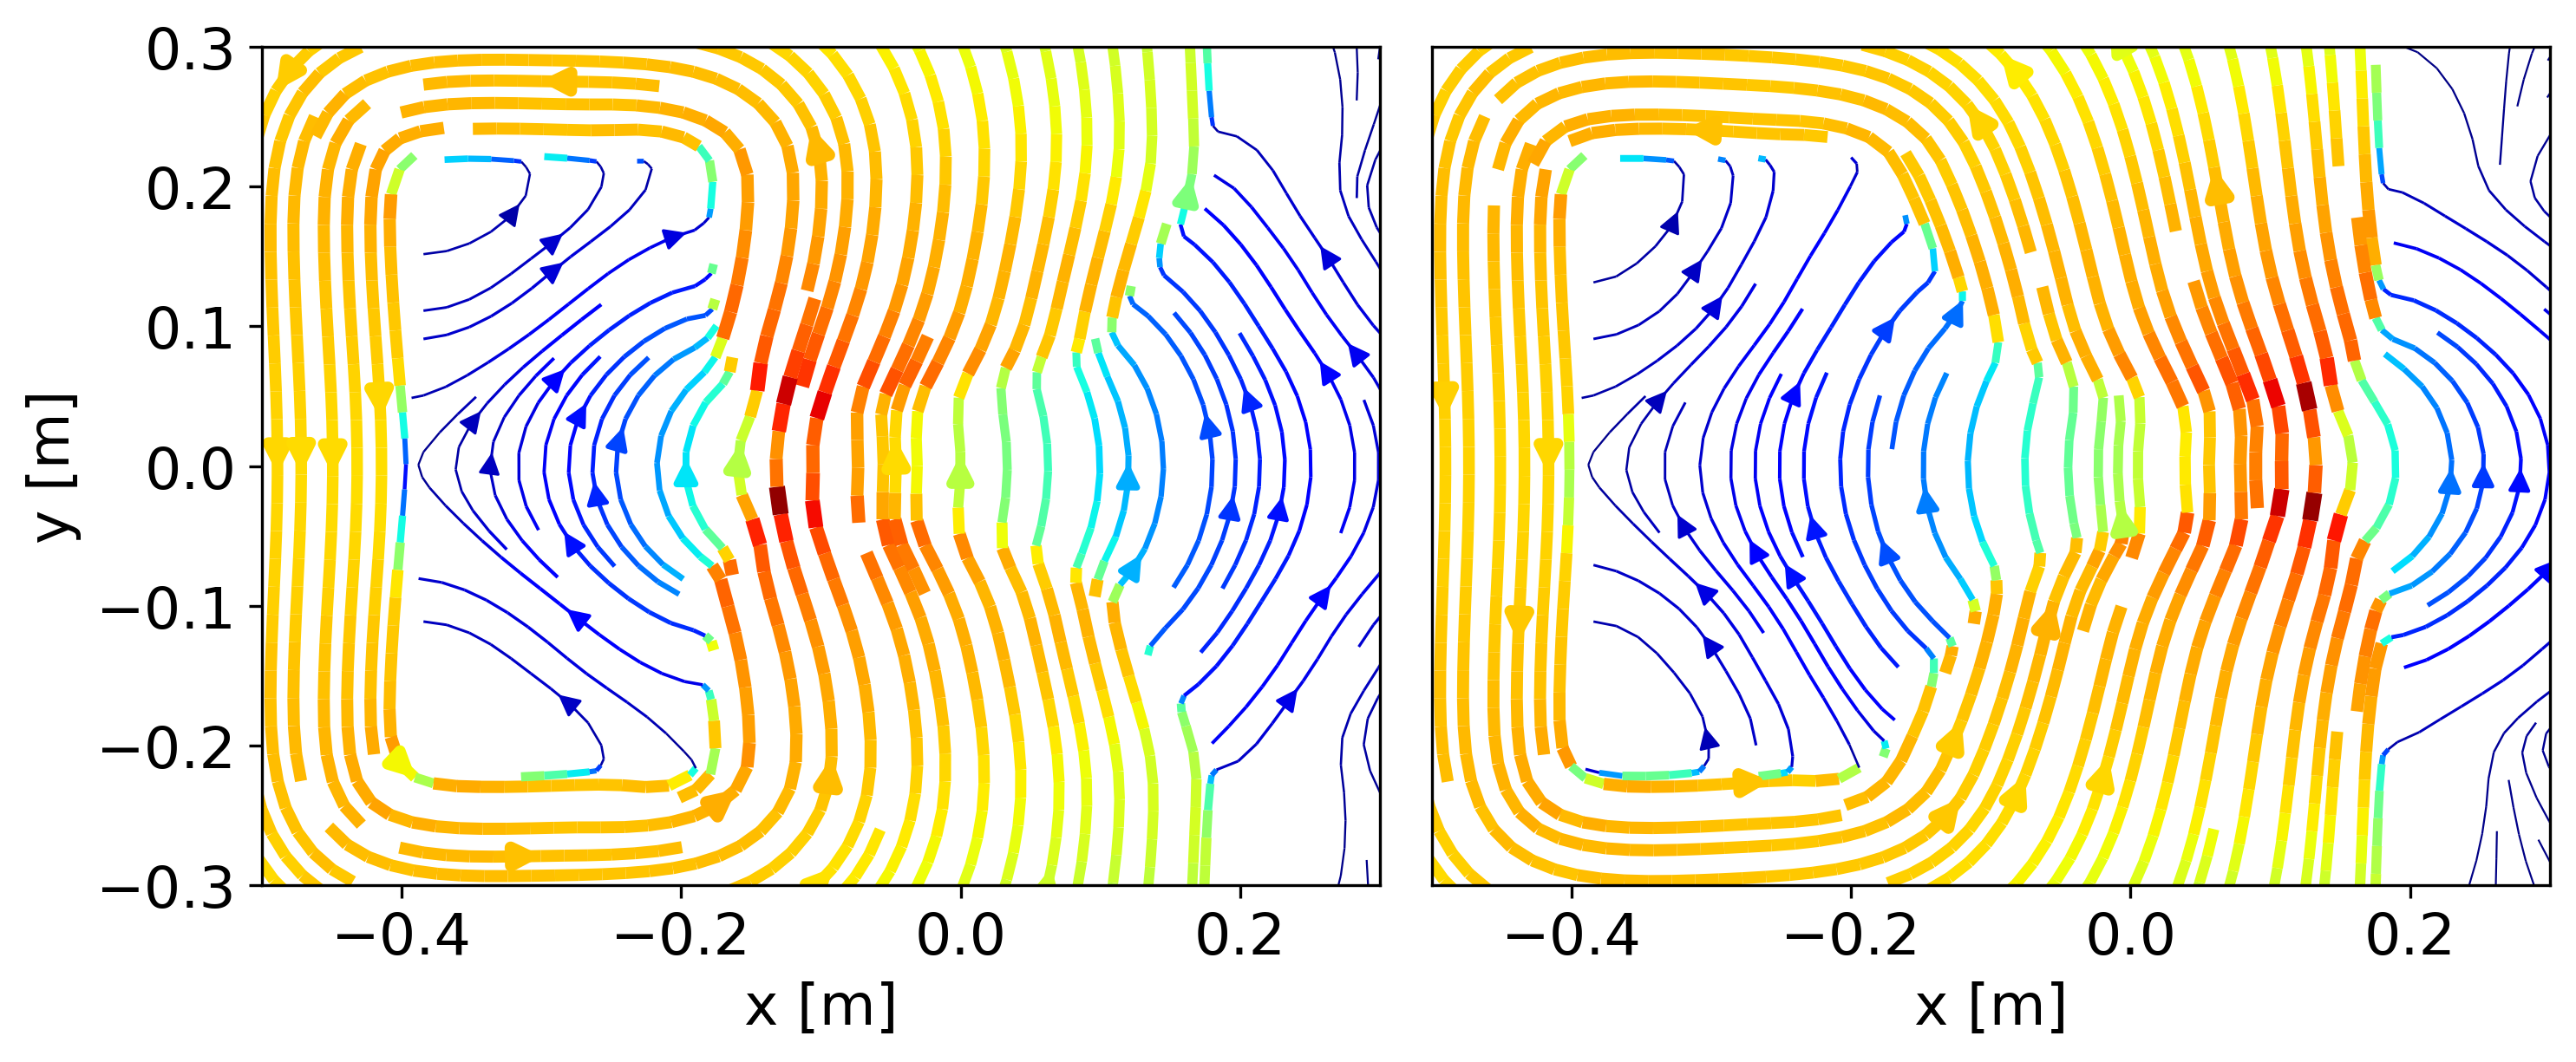
\includegraphics[width=0.7\textwidth]{01_Introduction/images/vector_flow.png}
\caption{Vector flow of an open defocusing block (left) and a closed focusing block (right).}
\label{fig:vector_flow}
\end{figure}

There are four magnets types: R, S, T and U, depending on the arrangement of the half-units (FD or DF) and whether the main coil is on the inside or outside of the ring. Additional coils named the Pole Face Windings (PFW) and Figure-of-eight Loop (F8L) are inserted between the yoke and the vacuum chamber to control the tune and chromaticity. Although the nominal field region of the combined function
magnet extends over a large part of the magnet aperture around the circulating beam orbit, see Fig, \ref{fig:dipole_gradient_components}, the injection and extraction trajectory of the beam travels through strong regions of fringing or stray field. This is a consequence of the PS not being built with straight sections long enough for injection or extraction, forcing the beam to travel through the stray fields of the MUs \cite{risselada_beam_nodate, johnson_beam_2022}.
 
\begin{figure}[H]
\centering
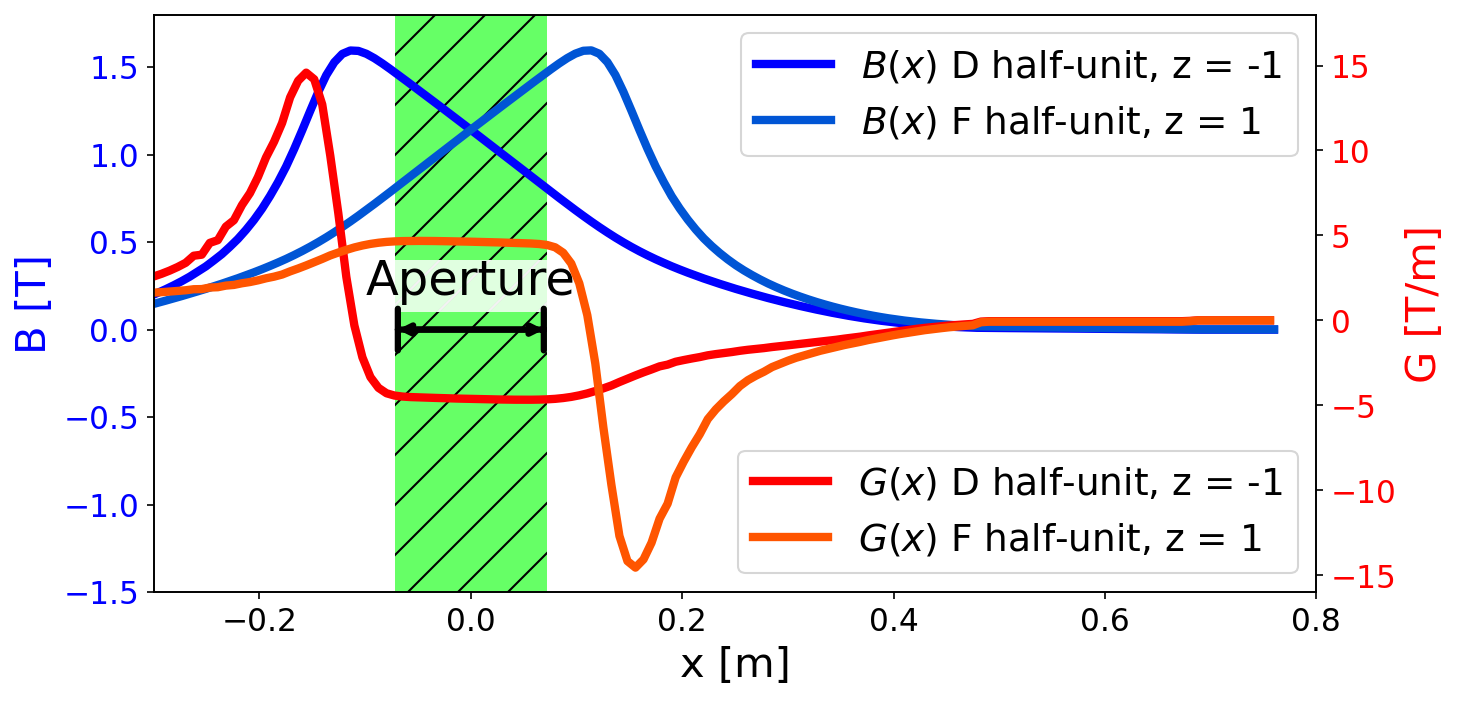
\includegraphics[width=0.7\textwidth]{01_Introduction/images/dipole_gradient_components.png}
\caption{Dipole and gradient component of a PS U-type MU centered in the vertical plane in both half-units at 24 GeV. The green-shaded region of 14.4 cm shows where the gradient is constant to within 5\% of the central and nominal gradient. A width similar to the beam pipe aperture in MU62 of 14.6 cm. Outside this region, the gradient is non-linear and, at its maximum, is almost three-fold higher in amplitude.}
\label{fig:dipole_gradient_components}
\end{figure}

\subsubsection{The OPERA model}

A finite element magnetic model of the PS MU was developed using Cobham's \texttt{Opera-3D}~\cite{noauthor_opera_nodate, anglada_pxmu_hrcwp_nodate} to generate field maps at different energies (different current in the main coils), different PFW, different F8L settings, and for all four magnet types. The model includes the main junction gap of \SI{20}{mm} (a significant source of fringe field) between the two half-units, as well as the mini junctions between open blocks of \SI{9.75}{mm} and \SI{7.75}{mm} between closed blocks. A plane containing the geometry of open and closed yokes is swept in the longitudinal direction, allowing us to maintain a high accuracy of the model and to reduce the computation time. This feature of a single plane also comes with limitations, as it models straight magnets, whilst real magnets have a curvature. The density of the mesh is adjusted so that it has a high resolution in close proximity to the central orbit and at the junctions to capture the fringe fields \cite{anglada_reference_2019}.

An example of a vector field map ($B_x$, $B_y$, $B_z$) in a Cartesian coordinate system ($x$,$y$,$z$) produced by the \texttt{Opera-3D} model is presented in Fig.~\ref{fig:dipole_field}. The transverse displacement of the peak of the vertical dipole field $B_{y}$ along the z-axis corresponds to the switch from one half-unit to the next. The resolution of the field map is high enough to see the mini-junction between the five blocks.

\begin{figure}[!htb]
   \centering
   %trim={<left> <lower> <right> <upper>}
   \includegraphics*[width=0.7\columnwidth, trim={0 2.9cm 0 4.3cm},clip]{01_Introduction/images/dipole_field.png}
   \caption{Dipole field map of a U-type magnet centered in the vertical plane at \SI{24}{GeV}.}
   \label{fig:dipole_field}
\end{figure}

The gradient is calculated from the dipole field component using the following formula:
 
$$ \boldsymbol{G}(x_{j},z) = \frac{\Delta\boldsymbol{B}}{\Delta x} = \frac{\boldsymbol{B}(x_{i+1},z) - \boldsymbol{B}(x_{i},z)}{x_{i+1}-x_{i}} $$
where:
$$ x_{j} = \frac{x_{i+1} + x_{i}}{{2}} $$

\subsubsection{Beam tracking}

Particle tracking through field maps is done using the Boris algorithm that tracks charged particles in EM fields using the discretised equation of motion of the Lorentz force \cite{dutheil_pybttrackersborispy_nodate,qin_why_2013,ripperda_comprehensive_2018}. Field maps were produced for each magnet type at three different energies: injection at \SI{2}{GeV} with \SI{533}{A}, slow extraction to the East Area at \SI{24}{GeV} with \SI{4642}{A}, and extraction to the SPS at \SI{26.4}{GeV} with \SI{5386}{A}. In the following, measurements and tracking studies of injection from the BTP transfer line to the PS and extraction from the PS to the East Area are discussed.


\subsubsection{Magnetic shims}

To counteract stray fields, magnetic shims are installed in MU16 (fast extraction to SPS) and MU63 (slow extraction to East Area) to homogenise the field by shielding the ejected beam from the non-linear fringe field \cite{zickler_influence_nodate}. In MU16, the shims have different radial positions for each of the five different shims, while in MU63, the vacuum pipe is covered with a constant rectangular shim. In MU62, no shims are installed, where the model predicts the most important stray field effect. In the next step, the shim geometry will be incorporated into the \texttt{OPERA-3D} model, which will significantly increase the computation time of the finite element solver due to the increased complexity of the geometries, but will allow for a more accurate representation of the actual stray fields. For detailled drawing, see Appendix \ref{magnetic shims}.


%\textbf{State clearly the efforts we are going to here to measure the beam parameters that come out of the machine and through the stray fields. State the quad scan technique and challenges with lack of instrumentation but that work continues with BTVs and additional of filter wheels for a comparison with simulation}





%\subsection{Previous studies done on the stray fields}

\subsection{Identifying Stray Field Locations in the PS}

Stray fields are particularly significant in regions where the magnetic gradient deviates from the nominal values, as shown in Figure \ref{fig:stray_field_loc}. This plot illustrates the gradient in the focusing part of a main unit (top) and the absolute gradient at various excursions (bottom). The top graph shows the gradient 
$G(x)$ as a function of the horizontal position x, highlighting significant deviations from the nominal value (\SI{4.63}{\Tesla\per\meter}) in specific regions. The data points correspond to different magnets, indicating where the gradient changes are most pronounced, specifically for MU62 and 63.
\\
\\
In the bottom graph, the nominal and actual gradients at the excursion points are compared. The blue bars represent the actual simulated gradients, while the red bars indicate the nominal values. Notably, magnets such as pr.bht63 and pr.bhu62 exhibit substantial discrepancies between the nominal and actual gradients, with the actual gradients being much more negative. This suggests strong stray fields in these areas.
\\
\\
These stray fields are expected to act most intensely at the injection and extraction points, specifically in the F16 and F61 lines. The deviations in gradient at these locations can significantly impact the beam quality and size. Understanding and mitigating these stray fields is crucial for maintaining optimal beam dynamics within the injection and extraction of the PS.

\begin{figure}[H]
\centering
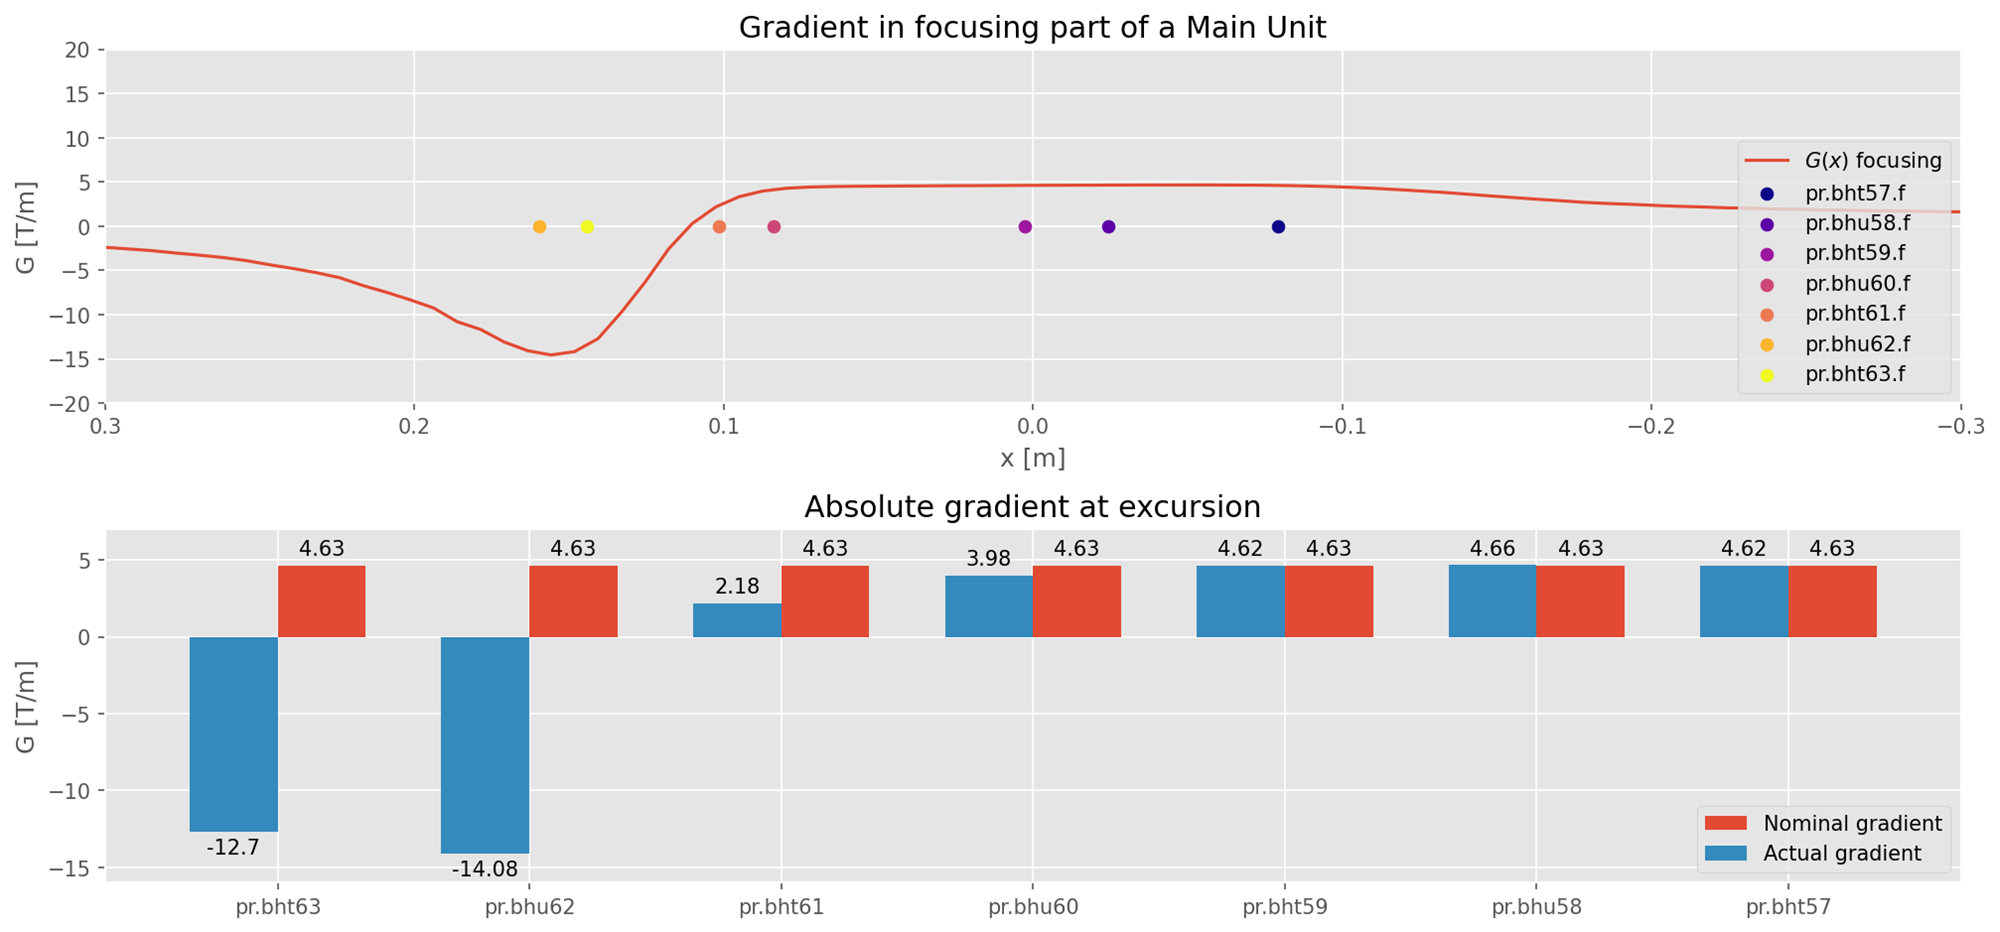
\includegraphics[width=1.0\textwidth]{01_Introduction/images/stray_field_location.png}
\caption{}
\label{fig:stray_field_loc}
\end{figure}

%\subsection{Shims (no shims in MU62 and shims in MU63)}